\chapter{Application d'un réseau de neurones à propagation directe}     % numéroté
\label{chap:Application}                   

\section{Présentation des données}
\label{sec:app:donnees}

On utilise la base de données  \verb@freMTPLfreq@ du paquetage \verb@CASdatasets@, \citep{cas}, pour la modélisation de la fréquence de réclamation. Ces données contiennent un portefeuille de \nombre{413169} polices d'assurance responsabilité civile automobile pour une compagnie d'assurance française.

Voici une brève description de chaque variable dans la base de données:
\begin{description}
\item[PolicyID] Identifiant de l'assuré \\
\item[ClaimNb]  Nombre de réclamation\\
\item[Exposure] Période durant laquelle la police d'assurance est effective, en année\\
\item[Power] Variable catégorielle ordonnée de la puissance du véhicule\\
\item[CarAge] Âge du véhicule, en année \\
\item[DriverAge] Âge du conducteur, en année\\
\item[Brand] Constructeur du véhicule  \\
\item[Gas] Type de carburant utilisé, régulier ou diésel\\
\item[Region] Région de la France\\
\item[Density] Nombre d'habitants par ${km}^2$ dans la ville où l'assuré réside \\
\end{description}

Il y a 421 observations qui ont une durée d'exposition plus grande qu'un an. Ces données sont corrigées à 1, puisqu'il s'agit probablement d'un erreur. 

On voit à la \autoref{fig:ClaimNbExpo} la répartition du nombre de réclamation. On a \nombre{14633} polices avec une réclamation, 726 avec deux réclamations, 28 avec trois réclamations et 3 avec quatre réclamations. On voit au graphique de droite de la \autoref{fig:ClaimNbExpo} la répartition du temps d'exposition. Une majorité des assurés de ce portefeuille ne sont pas assurés durant toute l'année. On a \nombre{29,54}\% des polices qui sont en vigueur toute l'année. 



\begin{figure}[b]
\caption{\label{fig:ClaimNbExpo} Nombre de réclamations observées (gauche), histogramme de l'exposition (droite).}
\centering
\begin{minipage}{0.4\linewidth}
\includegraphics[scale=0.5]{Graphiques/BarplotClaimNb}
\end{minipage}
\hfill
\begin{minipage}{0.4\linewidth}
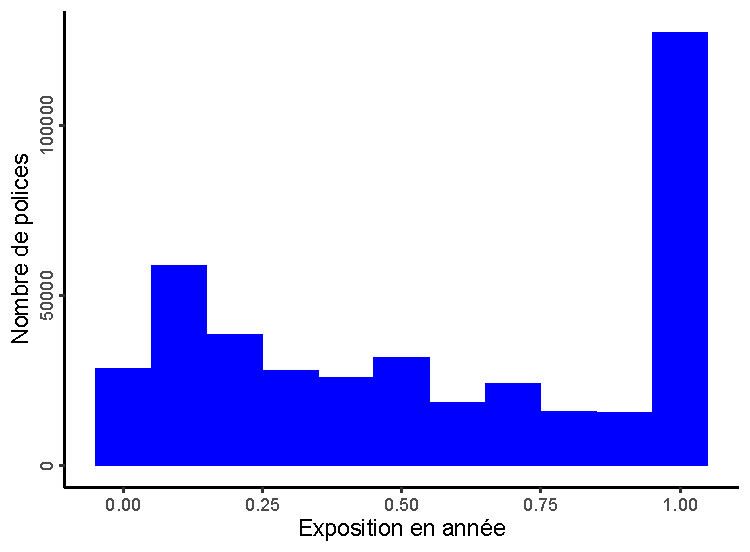
\includegraphics[scale=0.5]{Graphiques/RepartExposure}
\end{minipage}
\end{figure}

La \autoref{fig:ExpoTotFreqMoyRegion} montre la somme des expositions des assurés selon leur région de résidence et la fréquence moyenne observée par région. Une grande proportion de l'expérience du portefeuille provient de la région « Centre ». Il n'y a pas de grosse différence entre chaque région pour la fréquence moyenne observée. 


\begin{figure}
\caption{\label{fig:ExpoTotFreqMoyRegion} Exposition totale par région (gauche), fréquence moyenne observée par région (droite).}
\centering
\begin{minipage}{0.4\linewidth}
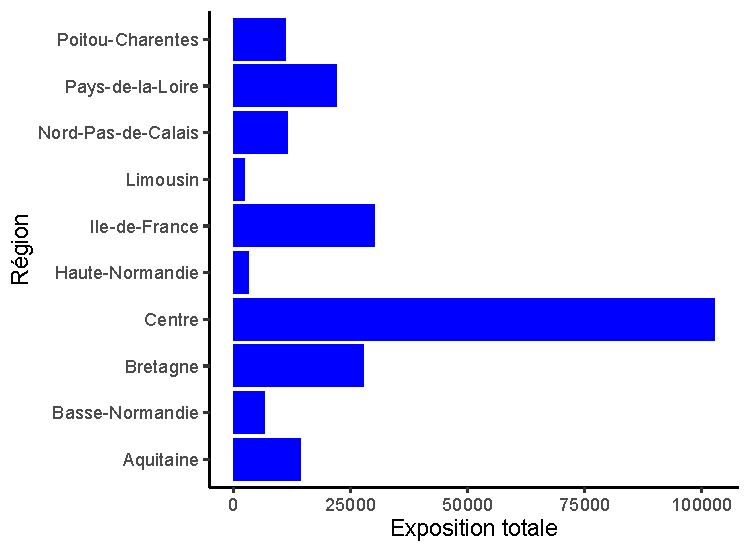
\includegraphics[scale=0.5]{Graphiques/ExpoTotRegion}
\end{minipage}
\hfill
\begin{minipage}{0.4\linewidth}
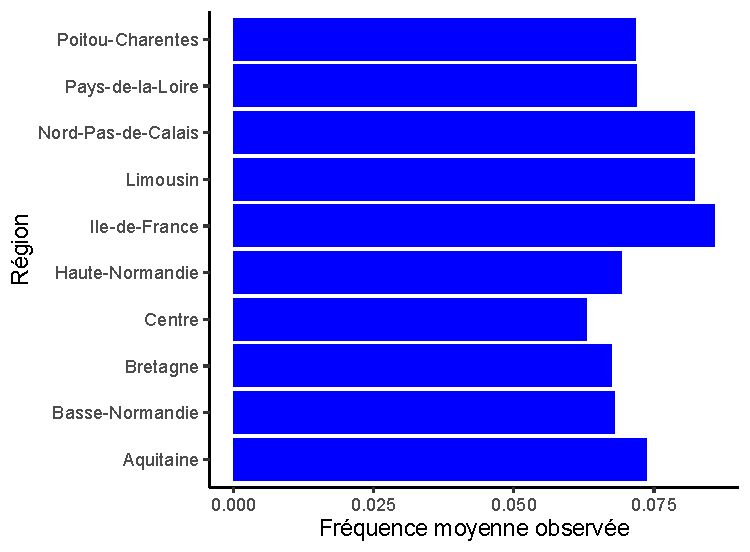
\includegraphics[scale=0.5]{Graphiques/FreqMoyRegion}
\end{minipage}
\end{figure}

La \autoref{fig:ExpoTotFreqMoyPower} montre la répartition de l'expérience en fonction de la catégorie du véhicule et leur fréquence moyenne observée. On voit une augmentation linéaire de la fréquence moyenne en fonction de la puissance du véhicule.

\begin{figure}
\caption{\label{fig:ExpoTotFreqMoyPower} Exposition totale par catégorie de véhicules (gauche), fréquence moyenne observée par catégorie de véhicule (droite).}
\begin{minipage}{0.4\linewidth}
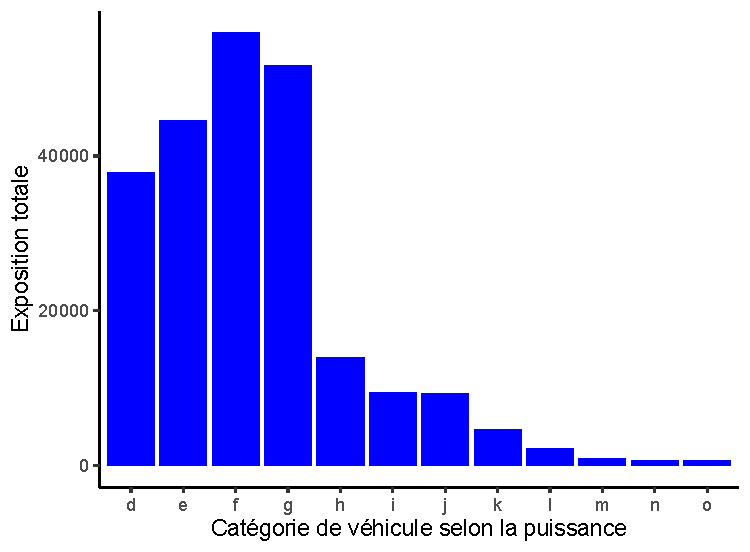
\includegraphics[scale=0.5]{Graphiques/ExpoTotPower}
\end{minipage}
\hfill
\begin{minipage}{0.4\linewidth}
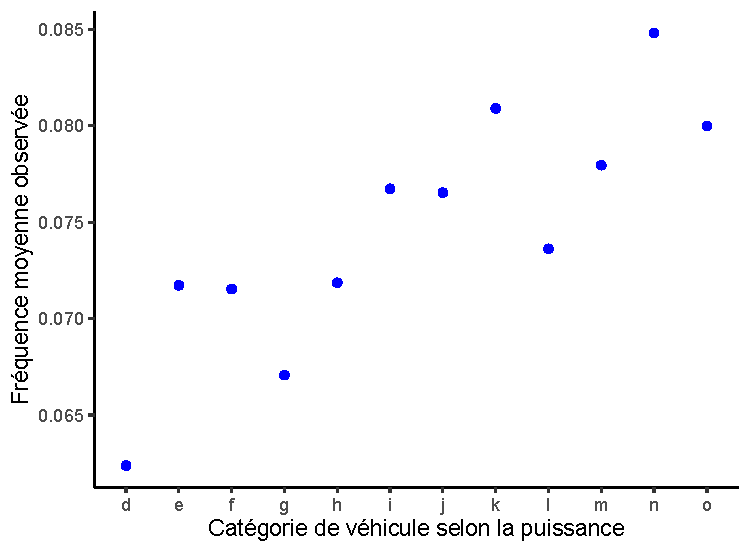
\includegraphics[scale=0.5]{Graphiques/FreqMoyPower}
\end{minipage}
\end{figure}

On observe à la \autoref{fig:ExpoTotFreqMoyCarAge} (droite) une légère augmentation de la fréquence moyenne observée pour l'âge du véhicule allant de 0 à environ 10. Par la suite, la fréquence diminue considérablement. À noter que les véhicules de 20 ans et plus ont été 
groupés. Ces véhicules représentent 8370 observations pour 2,026\% de la base de données.

\begin{figure}
\caption{\label{fig:ExpoTotFreqMoyCarAge} Exposition totale par âge du véhicule avec regroupement des véhicules de plus de 20 ans (gauche), fréquence moyenne observée par âge du véhicule (droite).}
\begin{minipage}{0.4\linewidth}
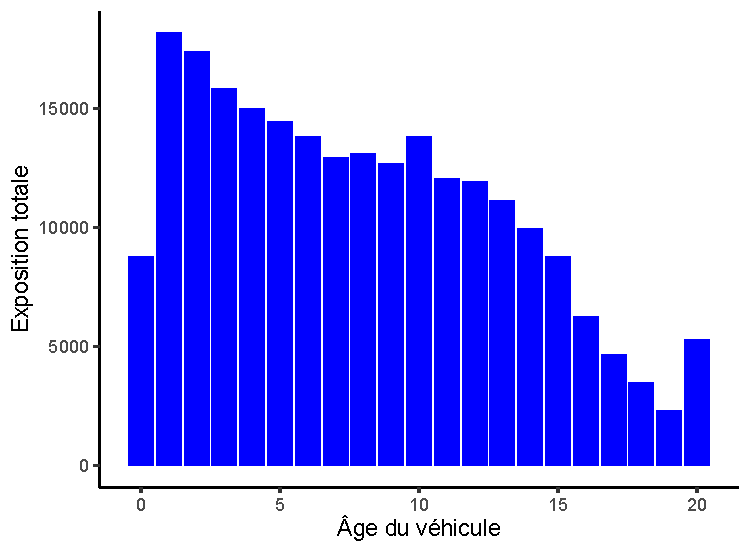
\includegraphics[scale=0.5]{Graphiques/ExpoTotCarAge}
\end{minipage}
\hfill
\begin{minipage}{0.4\linewidth}
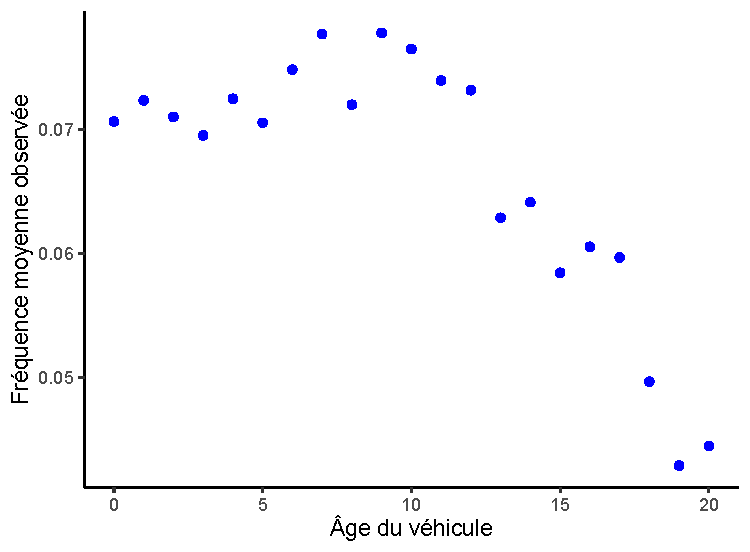
\includegraphics[scale=0.5]{Graphiques/FreqMoyCarAge}
\end{minipage}
\end{figure}

On remarque à la \autoref{fig:ExpoTotFreqMoyDriverAge} un mode autour de 50 ans. On remarque également que les assurés en bas de 25 ans font plus de réclamations. Il y a une légère augmentation de la fréquence moyenne autour de 45 ans. On voit également une variabilité de la fréquence observée pour les âges élevés. Cela est lié au fait qu'il y a peu d'observations (429) pour ces âges. Ainsi, on les regroupe en une catégorie 85 ans et plus.

\begin{figure}
\caption{\label{fig:ExpoTotFreqMoyDriverAge} Exposition totale par âge de l'assuré (gauche), fréquence moyenne observée par âge de l'assuré (droite).}
\begin{minipage}{0.4\linewidth}
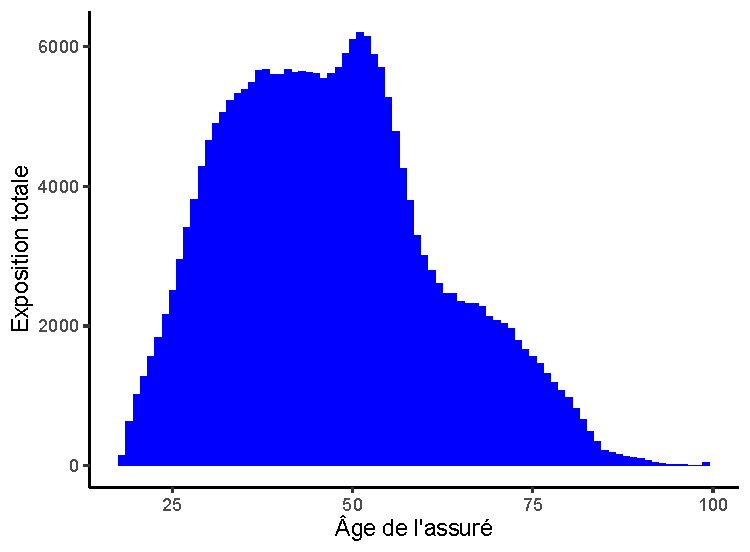
\includegraphics[scale=0.5]{Graphiques/ExpoTotDriverAge}
\end{minipage}
\hfill
\begin{minipage}{0.4\linewidth}
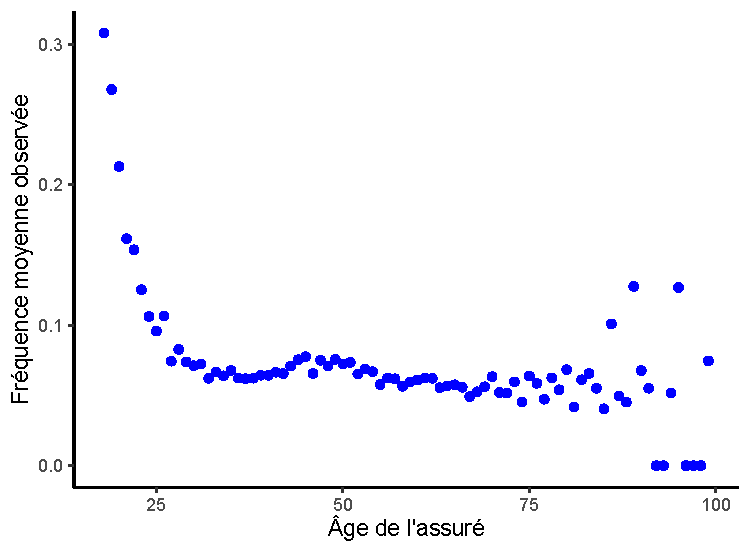
\includegraphics[scale=0.5]{Graphiques/FreqMoyDriverAge}
\end{minipage}
\end{figure}

\begin{figure}
\caption{\label{fig:ExpoTotFreqMoyBrand} Exposition totale par marque de véhicule (gauche), fréquence moyenne observée par marque de véhicule (droite).}
\begin{minipage}{0.4\linewidth}
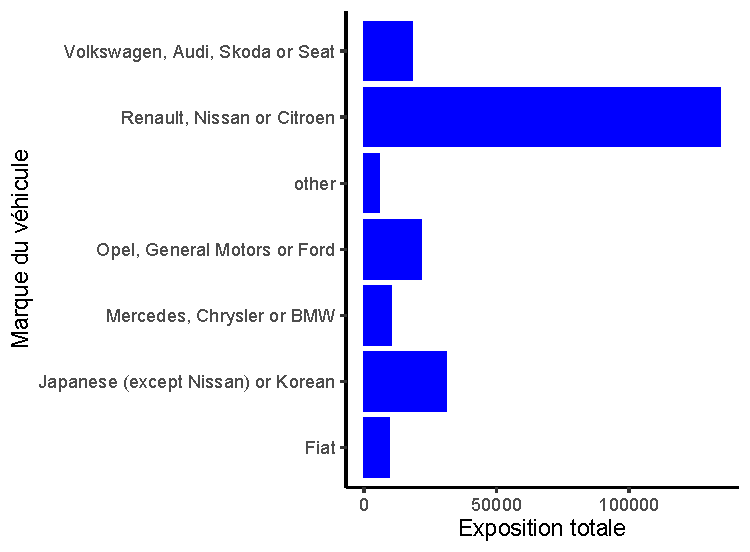
\includegraphics[scale=0.5]{Graphiques/ExpoTotBrand}
\end{minipage}
\hfill
\begin{minipage}{0.4\linewidth}
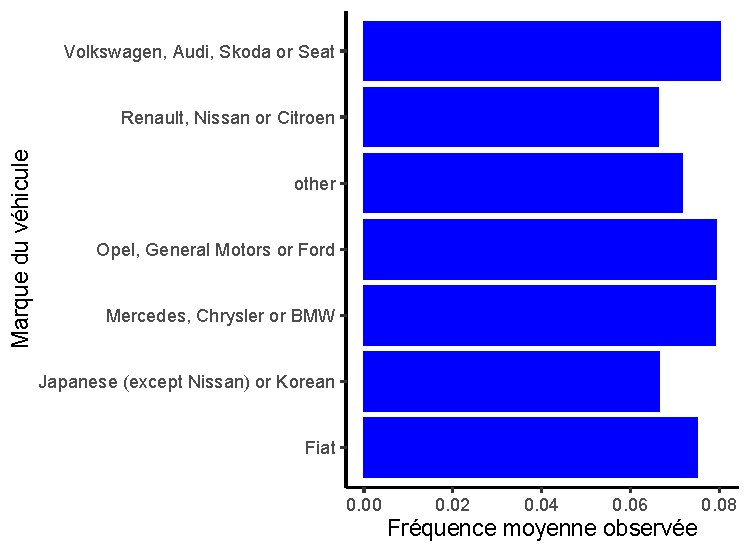
\includegraphics[scale=0.5]{Graphiques/FreqMoyBrand}
\end{minipage}
\end{figure}

\begin{figure}
\caption{\label{fig:ExpoTotFreqMoyGas} Exposition totale par type de carburant (gauche), fréquence moyenne observée par type de carburant (droite).}
\begin{minipage}{0.4\linewidth}
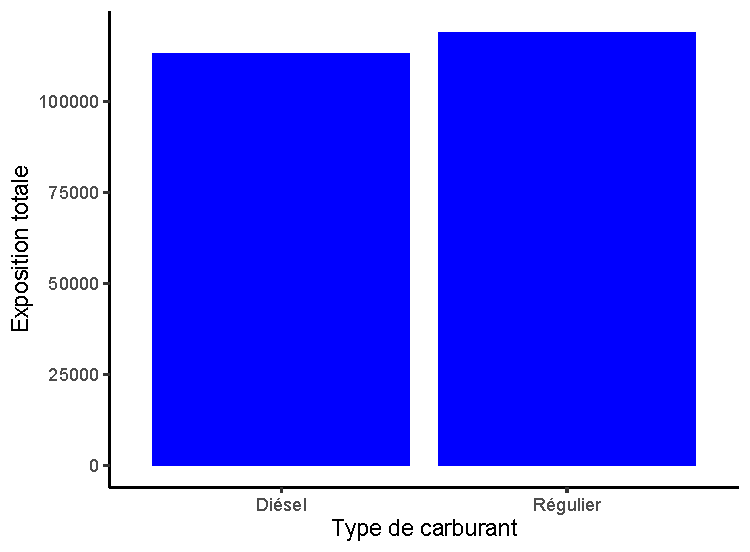
\includegraphics[scale=0.5]{Graphiques/ExpoTotGas}
\end{minipage}
\hfill
\begin{minipage}{0.4\linewidth}
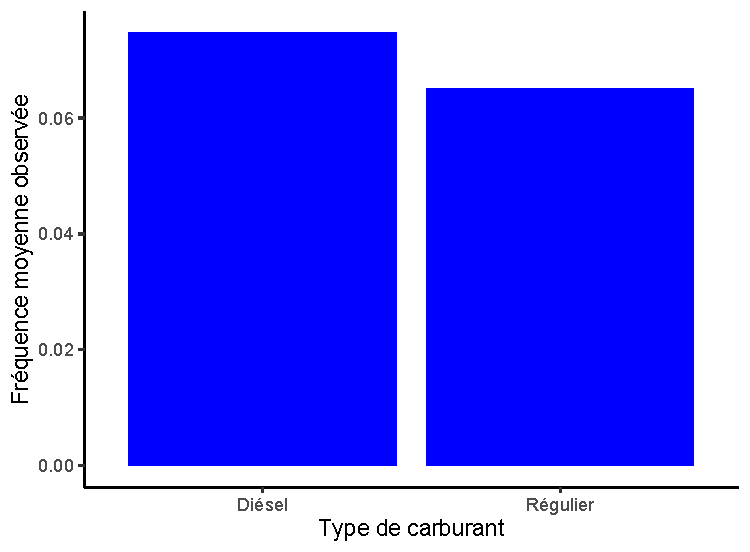
\includegraphics[scale=0.5]{Graphiques/FreqMoyGas}
\end{minipage}
\end{figure}




\section{Modèle de fréquence}
\label{sec:app:modele}

Pour chaque assuré $i$, on a un vecteur de sept dimensions qui représente la $i$\ieme observation:
\begin{align*}
x_i = \left( \text{Power}_i, \text{CarAge}_i, \text{DriverAge}_i, \text{Brand}_i, \text{Gas}_i,
 \text{Region}_i, \text{Density}_i \right)^\prime,\quad i = 1,\dots, 413169.
\end{align*}

On veut prédire $N_i= \verb=ClaimNb=_i \geq 0$ en tenant compte de l'exposition au risque, $v_i = \verb=Exposure=_i $, qui est différente d'un assuré à l'autre. On suppose que chaque observation est indépendante. On a que
\begin{align*}
N_i \sim Poisson\left(\lambda(x_i)v_i\right)
\end{align*}

On sépare les données en trois échantillons disjoints et en stratifiant sur la variable \verb=ClaimNb=. On utilise 60\% des données pour l'échantillon d'entrainement, $\mathcal{D}$, et 20\%  pour l'échantillon de test, $\mathcal{T}$, et l'échantillon de validation, $\mathcal{V}$. Au \autoref{tab:EchanClaimNb}, on voit que la proportion du nombre de réclamation est donc similaire entre chaque échantillon.

\begin{table}[b]
\centering
\caption{\label{tab:EchanClaimNb} Répartition du nombre de réclamations par échantillon}
\begin{tabular}{lrrrrr}
\toprule
 & \multicolumn{5}{c}{ \Verb=ClaimNb= (\%)}\\
\cmidrule{2-6}
Échantillon & 0 & 1 & 2 & 3 & 4\\
\midrule
Entrainement & 96.2751 & 3.5417 & 0.1759 & 0.0065 & 0.0008\\
Test & 96.2740 & 3.5421 & 0.1755 & 0.0073 & 0.0012\\
Validation & 96.2763 & 3.5410 & 0.1755 & 0.0073 & 0.0000\\
\bottomrule
\end{tabular}
\end{table}

On utilise la déviance de Poisson comme fonction de perte:
\begin{align*}
\mathcal{L}(\mathcal{D}, \lambda)=\frac{1}{n} \sum_{i=1}^{n} 2 N_{i}\left[\frac{\lambda\left(\boldsymbol{x}_{i}\right) v_{i}}{N_{i}}-1-\log \left(\frac{\lambda\left(\boldsymbol{x}_{i}\right) v_{i}}{N_{i}}\right)\right].
\end{align*} 

\section{Modèle de base}
\label{sec:modèledebase}

On construit un modèle de base pour pouvoir comparer les réseaux avec celui-ci. On considère un modèle linéaire généralisé Poisson avec le lien logarithmique. On suppose la relation suivante:
\begin{align*}
E\left[ \dfrac{N_i}{v_i} \right] = \exp\left\{ \mathbf{x_i} \boldsymbol\omega\right\}.
\end{align*}
 

On ajuste les données $\mathcal{D}$ à ce modèle. Pour le modèle de base, on considère seulement les effets principaux des variables explicatives. On ajuste le premier modèle suivant:
\begin{align*}
\log\left(\dfrac{\lambda_i}{v_i}\right) = b+ \omega_1 \text{\Verb=DriverAge=}_i + \omega_2 \text{\Verb=Power=}_i + \omega_3 \text{\Verb=CarAge=}_i + \omega_4 \text{\Verb=Region=}_i + \omega_5 \text{\Verb=Gas=}_i + \omega_6 \log\left\{\text{\Verb=Density=}_i\right\}.
\end{align*}

Pour la sélection de variable, on calcule la statistique de Wald pour chaque paramètre estimé. On observe les résultats au \autoref{tab:StatWaldglm1} obtenus à partir de la fonction \textbf{R}, \verb=summary=. La variable \verb=Region= ne semble pas être significative avec  deux niveaux qui obtiennent un seuil observé sous 5\% et seulement un niveau avec un seuil sous 1\%. On vérifie la pertinence de cette variable avec un test de vraisemblance et on retire la variable \verb=Region=. 

\begin{table}
\centering
\caption{\label{tab:StatWaldglm1} Seuil observé de la statistique de Wald pour les paramètres de glm1}
\begin{tabular}{lr}
\toprule
Variable & seuil observé\\
\midrule
(Intercept) & 0.0000000\\
Power & 0.0000025\\
CarAge & 0.0000001\\
DriverAge & 0.0000000\\
\addlinespace
Br.1 & 0.0000000\\
Br.2 & 0.6457504\\
Br.3 & 0.4977571\\
Br.4 & 0.1940670\\
Br.5 & 0.1329266\\
Br.6 & 0.6915220\\
\addlinespace
GasRegular & 0.0000000\\
Re.1 & 0.2459378\\
Re.2 & 0.0065408\\
Re.3 & 0.0560250\\
Re.4 & 0.6325997\\
\addlinespace
Re.5 & 0.1563482\\
Re.6 & 0.0264359\\
Re.7 & 0.5915649\\
Re.8 & 0.0579710\\
Re.9 & 0.5396968\\
\addlinespace
Density & 0.0000000\\
\bottomrule
\end{tabular}
\end{table}


\begin{table}
\centering
\caption{\label{tab:LRTglm1} Résultats des test du ratio de vraisemblance pour glm1}
\begin{tabular}{lrrr}
\toprule
  & Df & LRT & Pr(>Chi)\\
\midrule
Power & 1 & 21.83182 & 0.0000030\\
CarAge & 1 & 28.25304 & 0.0000001\\
DriverAge & 1 & 211.92967 & 0.0000000\\
Brand & 6 & 86.29772 & 0.0000000\\
Gas & 1 & 35.54875 & 0.0000000\\
\addlinespace
Region & 9 & 19.25317 & 0.0231243\\
$\log\{Density\}$ & 1 & 261.57895 & 0.0000000\\
\bottomrule
\end{tabular}
\end{table}



\section{Pré-traitement des données pour les réseaux de neurones}
\label{sec:app:pretraitement}

On doit traiter les variables avant d'entrainer les réseaux de neurones. Ceux-ci peuvent traiter seulement des variables numériques, ainsi on doit transformer les variables catégorielles. Les variables continues doivent, quant à elles, être standardisées. Cela permet d'avoir une performance plus rapide. %ajouter une source

\subsection{Traitement des variables catégorielles}

La variable \verb=Power= est transformée en facteur de 1 à 12. La variable \verb=Gas= est transformée en variable binaire, où \Verb@Regular@ $=1$ et \Verb@Diesel@ $=0$. Pour les variables \verb=Region= et \verb=Brand=, on utilise deux façons de les traiter et on compare leurs résultats dans l'analyse. La première façon est de créer ($k-1$) variables binaires pour une variable catégorielle avec $k$ niveaux. 

La deuxième méthode qu'on utilise est une technique d'apprentissage de la représentation ( « representation learning » ). Il s'agit d'ajouter des couches de plongement ( « embedding layers» ) au réseau qui permettent de réduire la dimension de ces variables catégorielles, voir \citet{richman2018ai}.


En appliquant la première méthode, on obtient un vecteur de variables explicatives de 20 dimensions
\begin{align*}
\mathcal{X} \subset[1,12] \times\{0,1\} \times\{0,1\}^{7} \times\{0,1\}^{9} \times[0,100] \times[0,90] \times[2,27000].
\end{align*}

La deuxième méthode permet de réduire la dimension de \verb=Region= et \verb=Brand= à $d=2$ et ainsi on obtient un vecteur de variables explicatives de 9 dimensions. 





\subsection{Traitement des variables continues}
\label{subsec:TraitementVarContinues}

Premièrement, on applique la transformation $log$ à la variable \verb=Density=. Par la suite, on doit s'assurer que chaque variable soit sur la même échelle. On utilise la transformation suivante pour les variables \verb=DriverAge=, \verb=CarAge=, \verb=Power= et \verb=log(Density)=:
\begin{align*}
\frac{x_i-\min (x_i)}{\max (x_i)-\min (x_i)} \mapsto [0,1].
\end{align*}

\section{Réseaux utilisés}
\label{sec:app:reseauxutilisés}

On détaille dans cette section la démarche utilisée pour construire les différents modèles. 

Tout d'abord, on fera une distinction entre les réseaux à une seule couche cachée et ceux à plusieurs couches cachées. Selon %source
, les réseaux de neurones à une seule couche sont capables d'approximer n'importe quelle fonction non linéaire. On verra toutefois que le fait d'ajouter des couches cachées au réseau permet d'apprendre les interactions entre les variables explicatives plus efficacement. Ensuite, on compare la différence entre les réseaux utilisant l'approche des variables binaires et les réseaux utilisant l'approche des couches de plongement. %Finalement on parle de la méthode Cann

On utilise le paquetage \verb=keras= qui est une interface au logiciel du même nom, \citep{keras}.
Comme mentionné à la section 4 de \citet{ferrario2018insights}, on est pas intéressé à trouver le minimum total de $\mathcal{L}(\mathcal{D}, \hat{\lambda})$ étant donné de la sur-paramétrisation des réseaux. L'idée est d'arrêter au bon moment l'algorithme de rétro-propagation. On y arrive en établissant une règle d'arrêt qui sera la même pour tous les réseaux ajustés. On arrête l'entrainement lorsque l'erreur de validation ne s'est pas améliorée depuis 20 epochs et on demande au modèle de retourner les paramètres qui permettent d'obtenir la plus petite erreur de validation. De cette façon, on s'assure de ne pas surajuster le modèle. Le \autoref{code:regleArret} montre comment on implémente cela avec \verb=keras=. De plus, pour chaque réseau on utilise, évidemment, le même échantillon de validation $\mathcal{V}$. On fixe la taille de mini-lot ( « mini-batch » ) à 8192. On établit un taux de réduction du taux d'apprentissage de 0.05. Ainsi, lorsque l'erreur de validation ne s'est pas améliorée depuis 10 epochs, on obtient un taux d'apprentissage 20 fois plus petit que le précédant. Cela permet à l'algorithme de tenter de quitter des points de selle, où le gradient de la fonction de perte est nul ou presque.% ajouter une référence


\begin{lstlisting}[caption= {Définition des paramètres de l'algorithme},label=code:regleArret]
	model %>% fit(list(XlearnNN, WlearnNN), 
              	YlearnNN,
              	validation_data = list(list(XvalNN,WvalNN),YvalNN),
              	epochs = 1000, 
              	batch_size = 8192,
              	callbacks = list(callback_early_stopping(patience = 20, 
              			restore_best_weights = T),
              	callback_reduce_lr_on_plateau(factor = 0.05)
              	)
              	)
\end{lstlisting}



\subsection{Réseau de neurones « shallow »}
\label{subsec:Shallow}

Comme mentionné précédemment, on ne cherche pas à trouver \emph{le} meilleur modèle, mais bien \emph{un} des meilleurs modèles. Ainsi, la méthode utilisée pour trouver les hyperparamètres du modèle final vise à améliorer une structure de base avec certains hyperparamètres. Cette structure de base se traduit par le nombre de neurones dans la couche cachée que l'on fixe. Le \autoref{tab:resultsShallow} montre l'erreur de validation pour $q_1 \in \left\{8, 16, 32, 64, 128 ,256 ,512\right\}$ avec la règle d'arrêt mentionnée antérieurement. On fixe donc le nombre de neurones à 32 et on tente d'optimiser le taux d'abandon, $d$, et les taux de régularisation, $\ell_2$ et $\ell_2$, à l'aide d'une grille de recherche disponible au \autoref{tab:rechercheShallow} de l'\autoref{ann:grilleRecherche}.

\begin{table}
\centering
\caption{\label{tab:resultsShallow} Résultats de la recherche du nombre de neurones pour le réseau avec une couche cachée}
\begin{tabularx}{0.6\textwidth}{Xrrr}
\toprule
Nombre \newline de neurones & $\mathcal{L}\left\{\mathcal{V},\hat{\lambda} \right\} $ & $\mathcal{L}\left\{\mathcal{D},\hat{\lambda} \right\} $ &  Epochs\\
\midrule
32 & \textbf{0.2511} & 0.2503 & 51\\
64 & 0.2516 & 0.2512 & 58\\
16 & 0.2518 & 0.2523 & 45\\
512 & 0.2519 & 0.2490 & 33\\
256 & 0.2519 & 0.2496 & 37\\
\addlinespace
128 & 0.2520 & 0.2510 & 33\\
8 & 0.2521 & 0.2523 & 100\\
\bottomrule
\end{tabularx}
\end{table}


On présente les six meilleurs résultats dans le \autoref{tab:resultsShallow32}. Le réseau qui offre la plus petite erreur de validation est celui avec $d=0.25$. On remarque qu'aucun des trois meilleurs modèles n'inclut une régularisation $\ell_1$ ou $\ell_2$. Une grille de recherche plus grande aurait peut-être permis de diminuer l'erreur à l'aide d'autres valeurs pour les taux de régularisation. On se limite à ces valeurs par souci de temps. Toutefois, on verra à l'aide des autres modèles que le taux d'abandon offre de meilleurs résultats , et ce  plus efficacement que les taux de régularisation.


\begin{table}
\centering
\caption[Résultats du réseau d'une couche cachée avec 32 neurones]{\label{tab:resultsShallow32} Résultats de la recherche des hyperparamètres pour le réseau de neurone d'une couche cachée avec 32 neurones}
\begin{tabular}{rrrrrr}
\toprule
$\mathcal{L}\left\{\mathcal{V},\hat{\lambda} \right\} $ & $\mathcal{L}\left\{\mathcal{D},\hat{\lambda} \right\} $ & $d$ & $\ell_1$ & $\ell_2$ & Epochs\\
\midrule
\textbf{0.2508} & 0.2512 & 0.25 & 0 & 0 & 66\\
0.2510 & 0.2518 & 0.50 & 0 & 0 & 70\\
0.2510 & 0.2504 & 0.00 & 0 & 0 & 54\\
0.2511 & 0.2519 & 0.50 & 0 & 0.001 & 79\\
0.2513 & 0.2520 & 0.25 & 0.001 & 0.001 & 82\\
0.2514 & 0.2526 & 0.50 & 0.001 & 0.001 & 125\\
\bottomrule
\end{tabular}
\end{table}

\subsection{Réseau à deux couches cachées}
\label{subsec:deep2}

On utilise la même méthode que pour le réseau à une couche cachée. On tente de fixer le nombre de neurones par couche en premier. On cherche parmi une combinaison de $q_1 \in \left\{ 8, 16, 32, 64 \right\}$, et $q_2\in \left\{8,16,32,64 \right\}$. On obtient les résultats au \autoref{tab:ResultsDeep2}. La combinaison $(q_1,q_2) = (8,8)$ donne la plus petite erreur de validation. Cependant, on tente également d'optimiser le modèle avec $(q_1,q_2)=(32,16)$. L'erreur d'entrainement pour cette combinaison est largement inférieure à $(q_1,q_2) = (8,8)$ et le nombre d'epochs est plus bas. Il est probable que le nombre plus élevé de paramètres fasse en sorte qu'il surajuste rapidement les données d'entrainement et, ainsi, l'algorithme exerce la règle d'arrêt rapidement. On peut donc penser que ce réseau pourrait bénéficier d'une régularisation quelconque. Ainsi, on fait une grille de recherche pour les deux réseaux mentionnés des hyperparamètres $d_1$, $d_2$, $\ell_1$ et $\ell_2$. Les valeurs de la grille sont au \autoref{tab:rechercheDeep2} de l'\autoref{ann:grilleRecherche}. On utilise les mêmes taux de régularisation sur les deux couches cachées, mais on utilise deux taux d'abandon différents.  Le \autoref{code:deep2} montre aux lignes  3 et 7 qu'on utilise \verb=FLAGS$l1= et \verb=FLAGS$l2= à chaque couche. On utilise également des couches de normalisation, aux lignes 4 et 8, qui permettent de standardiser la sortie de chaque neurone de la couche précédente. Cela permet d'éviter le problème de gradient disparaissant.%ajouter source


\begin{table}
\centering
\caption{\label{tab:ResultsDeep2} Résultats de la recherche du nombre de neurones par couche pour le réseau avec deux couches cachées}
\begin{tabularx}{0.6\textwidth}{Xrrr}
\toprule
Nombre \newline de neurones & $\mathcal{L}\left\{\mathcal{V},\hat{\lambda} \right\} $ & $\mathcal{L}\left\{\mathcal{D},\hat{\lambda} \right\} $ & Epochs\\
\midrule
(8, 8) & \textbf{0.2512} & 0.2510 & 64\\
(32, 16) & \textbf{0.2514} & 0.2496 & 46\\
(16, 32) & 0.2514 & 0.2504 & 55\\
(16, 16) & 0.2516 & 0.2505 & 54\\
(16, 64) & 0.2517 & 0.2502 & 49\\
(32, 32) & 0.2517 & 0.2498 & 44\\
\bottomrule
\end{tabularx}
\end{table}

\begin{lstlisting}[caption = {Définition de la structure du réseau à deux couches cachées}, label= code:deep2]
 net <- features.0 %>%
  layer_dense(units = FLAGS$hidden1,activation="relu",kernel_initializer = initializer_he_normal(seed=2L),
              kernel_regularizer = regularizer_l1_l2(l1 = FLAGS$l1, l2 = FLAGS$l2)) %>% 
  layer_batch_normalization() %>%
  layer_dropout(rate=FLAGS$dropout1) %>% 
  layer_dense(units = FLAGS$hidden2,activation="relu",kernel_initializer = initializer_he_normal(seed=3L),
              kernel_regularizer = regularizer_l1_l2(l1 = FLAGS$l1, l2 = FLAGS$l2)) %>% 
  layer_batch_normalization() %>%
  layer_dropout(rate=FLAGS$dropout2) %>% 
  layer_dense(units=1, activation='linear', 
              weights=list(array(0, dim=c(FLAGS$hidden2,1)), 
              	array(log(lambda.hom), dim=c(1))))
\end{lstlisting}


On présente les six meilleurs réseaux au \autoref{tab:ResultsDeep2Tuning}.  On sélectionne le modèle avec 32 et 16 neurones et $d_2=0.25$. Encore une fois, on remarque qu'aucun des meilleurs modèles ne contient une régularisation $\ell_1$ ou $\ell_2$.

\begin{table}
\centering
\caption{\label{tab:ResultsDeep2Tuning}Résultats de la recherche des hyperparamètres pour les réseaux à deux couches cachées}
\begin{tabularx}{0.8\textwidth}{Xrrrrrrr}
\toprule
Nombre \newline de neurones & $\mathcal{L}\left\{\mathcal{V},\hat{\lambda} \right\} $ & $\mathcal{L}\left\{\mathcal{D},\hat{\lambda} \right\} $ & $d_1$ & $d_2$ & $\ell_1$ & $\ell_2$ & Epochs\\
\midrule
(32, 16) & \textbf{0.2510} & 0.2504 & 0.00 & 0.25 & 0 & 0 & 56\\
(32, 16) & 0.2510 & 0.2511 & 0.25 & 0.25 & 0 & 0 & 72\\
(8, 8) & 0.2511 & 0.2515 & 0.00 & 0.25 & 0 & 0 & 76\\
(32, 16) & 0.2511 & 0.2503 & 0.00 & 0.25 & 0 & 0 & 57\\
(32, 16) & 0.2511 & 0.2511 & 0.25 & 0.00 & 0 & 0 & 111\\
(8, 8) & 0.2512 & 0.2524 & 0.00 & 0.50 & 0 & 0 & 80\\
\bottomrule
\end{tabularx}
\end{table}

\subsection{Réseau à trois couches cachées}
\label{subsec:Deep3}

Pour le réseau à trois couches cachées, on teste d'abord le nombre de neurones par couche avec la combinaison des paramètres suivants: $q_1\in \left\{8, 16, 32 \right\}$, $q_2 \in \left\{8, 16, 32 \right\}$ et $q_3\in \left\{8, 16, 32 \right\}$. Un total de 27 possibilités sont testées. On présente les six meilleurs résultats au \autoref{tab:ResultsDeep3}. Pour les mêmes raisons énumérées à la \autoref{subsec:deep2}, on tente d'optimiser les hyperparamètres des modèles $(q_1,q_2,q_3) = (8,8,8)$ et $(q_1,q_2,q_3) = (32,16,8)$. 
Par souci de temps, on tente d'optimiser d'abord $d_1$ et $d_2$ pour ensuite tenter d'ajouter une régularisation $\ell_1$ ou $\ell_2$. À noter qu'on n'ajoute pas de taux d'abandon à la troisième couche cachée pour économiser le temps de calcul. On utilise la grille de recherche au \autoref{tab:rechercheDeep3} de l'\autoref{ann:grilleRecherche}. 

\begin{table}[b]
\centering
\caption{\label{tab:ResultsDeep3} Résultats de la recherche du nombre de neurones par couche pour le réseau avec trois couches cachées}
\begin{tabularx}{0.6\textwidth}{Xrrr}
\toprule
Nombre \newline de neurones & $\mathcal{L}\left\{\mathcal{V},\hat{\lambda} \right\} $ & $\mathcal{L}\left\{\mathcal{D},\hat{\lambda} \right\} $ & Epochs\\
\midrule
(8, 8, 8) & \textbf{0.2513} & 0.2507 & 72\\
(8, 8, 16) & 0.2519 & 0.2508 & 63\\
(32, 8, 8) & 0.2520 & 0.2501 & 35\\
(16, 8, 8) & 0.2520 & 0.2500 & 49\\
(32, 8, 16) & 0.2521 & 0.2500 & 46\\
\addlinespace
(32, 16, 8) & \textbf{0.2521} & \textbf{0.2492} & 37\\
\bottomrule
\end{tabularx}
\end{table}

Les résultats du \autoref{tab:ResultsDeep3Tuning} montrent que le réseau $(q_1,q_2,q_3)=(32,16,8)$ avec un taux d'abandon $d_2=0.5$ obtient la plus petite erreur de validation. 

\begin{table}
\centering
\caption{\label{tab:ResultsDeep3Tuning}Résultats de la recherche des hyperparamètres pour le réseau à trois couches cachées}
\begin{tabularx}{0.8\textwidth}{Xrrrrrrr}
\toprule
Nombre \newline de neurones & $\mathcal{L}\left\{\mathcal{V},\hat{\lambda} \right\} $ & $\mathcal{L}\left\{\mathcal{D},\hat{\lambda} \right\} $ & $d_1$ & $d_2$ & $\ell_1$ & $\ell_2$ & Epochs\\
\midrule
(32, 16, 8) & 0.2510 & 0.2511 & 0.00 & 0.50 & 0 & 0 & 72\\
(8, 8, 8) & 0.2511 & 0.2523 & 0.25 & 0.25 & 0 & 0 & 59\\
(8, 8, 8) & 0.2512 & 0.2514 & 0.00 & 0.25 & 0 & 0 & 83\\
(32, 16, 8) & 0.2512 & 0.2513 & 0.25 & 0.00 & 0 & 0 & 54\\
(8, 8, 8) & 0.2513 & 0.2517 & 0.25 & 0.00 & 0 & 0 & 59\\
\addlinespace
(32, 16, 8) & 0.2515 & 0.2528 & 0.50 & 0.25 & 0 & 0 & 71\\
\bottomrule
\end{tabularx}
\end{table}

\subsection{Réseau à quatre couches cachées}
\label{subsec:deep4}

Comme à la \autoref{subsec:Deep3}, on cherche d'abord quelle combinaison de neurones par couches cachées permet d'obtenir la plus petite erreur de validation parmi $q_1 \in \left\{8, 16, 32 \right\}$, $q_2 \in \left\{8, 16, 32 \right\}$, $q_3 \in \left\{8, 16\right\}$ et $q_4 \in \left\{8, 16 \right\}$. On fait ensuite une grille de recherche pour les hyperparamètres $d_1$, $d_2$ et $d_3$. Finalement, on optimise les hyperparamètres $\ell_1$ et $\ell_2$ par une autre grille de recherche, voir \autoref{tab:rechercheDeep4}. 

\begin{table}
\centering
\caption{\label{tab:ResultsDeep4} Résultats de la recherche du nombre de neurones par couche pour le réseau avec quatre couches cachées}
\begin{tabularx}{0.6\textwidth}{Xrrr}
\toprule
Nombre \newline de neurones & $\mathcal{L}\left\{\mathcal{V},\hat{\lambda} \right\} $ & $\mathcal{L}\left\{\mathcal{D},\hat{\lambda} \right\} $ & Epochs\\
\midrule
(16,16,16,16) & 0.2523 & 0.2501 & 34\\
(16,16,16,8) & 0.2524 & 0.2502 & 37\\
(16,32,16,16) & 0.2525 & 0.2494 & 35\\
(16,16,8,8) & 0.2525 & 0.2509 & 32\\
(16,32,8,16) & 0.2526 & 0.2489 & 42\\
\addlinespace
(16,8,16,8) & 0.2526 & 0.2513 & 42\\
\bottomrule
\end{tabularx}
\end{table}

\begin{table}
\centering
\caption{\label{tab:ResultsDeep4Tuning}Résultats de la recherche des hyperparamètres pour le réseau à quatre couches cachées}
\begin{tabularx}{0.9\textwidth}{Xrrrrrrrr}
\toprule
Nombre \newline de neurones & $\mathcal{L}\left\{\mathcal{V},\hat{\lambda} \right\} $ & $\mathcal{L}\left\{\mathcal{D},\hat{\lambda} \right\} $ & $d_1$ & $d_2$ & $d_3$ & $\ell_1$ & $\ell_2$ & Epochs\\
\midrule
(16,32,8,16) & 0.2514 & 0.2511 & 0.0 & 0.0 & 0.5 & 0e+00 & 0 & 133\\
(16,32,8,16) & 0.2515 & 0.2507 & 0.0 & 0.0 & 0.5 & 0e+00 & 0 & 98\\
(16,16,16,16) & 0.2517 & 0.2529 & 0.5 & 0.0 & 0.0 & 0e+00 & 0 & 67\\
(16,16,16,16) & 0.2517 & 0.2526 & 0.5 & 0.0 & 0.0 & 0e+00 & 0 & 66\\
(16,32,8,16) & 0.2517 & 0.2511 & 0.0 & 0.0 & 0.5 & 1e-06 & 0 & 98\\
\addlinespace
(16,16,16,16) & 0.2518 & 0.2523 & 0.0 & 0.5 & 0.0 & 0e+00 & 0 & 62\\
\bottomrule
\end{tabularx}
\end{table}

\subsection{Réseaux Cann et réseaux avec couches de plongement}
\label{subsec:CannEmbed}

Par souci de temps, les réseaux Cann et les réseaux avec couches de plongement n'ont pas été optimisés au niveau de leurs hyperparamètres. On a utilisé les valeurs trouvées à l'aide des réseaux simples. On optimise seulement le nombre d'epochs à l'aide de la même règle d'arrêt. On présente les résultats finaux au \autoref{tab:resultsTOT} classés en ordre de performance. On constate que tous les modèles performent mieux que le modèle de base. Un autre constat est que les couches de plongement améliorent la performance. En effet, tous les six meilleures modèles sont des modèles avec des couches de plongement.  Le seul modèle qui semble s'approcher de la performance est le Shallow, qui arrive à battre les modèles à quatre couches et couches de plongement. Cependant, pour les trois types de modèles, la structure qui performent le moins est celle avec quatre couches. Ainsi, le Shallow bat les modèles à quatres couches par défaut. C'est probablement l'inverse qui se produit, soit qu'une structure à quatre couches est trop complexe pour ce problème.

Une autre importante information qu'on retire de ces résultats est le fait que les modèles Cann sont plus performant que les modèles avec plongement pour chaque structure. L'initialisation par le Glm permet donc d'améliorer  les modèles avec constance.   


\begin{table}
\centering
\caption{\label{tab:resultsTOT} Résultats de l'erreur sur les données de test pour tous les modèles}
\begin{tabular}{lrrrr}
\toprule
Modèle & $\mathcal{L}\left\{\mathcal{T},\hat{\lambda} \right\} $ & $\mathcal{L}\left\{\mathcal{D},\hat{\lambda} \right\} $ & $\mathcal{L}\left\{\mathcal{V},\hat{\lambda} \right\} $ & Epochs\\
\midrule
CannDeep3 & 0.25049 & 0.25086 & 0.25064 & 78\\
Deep3Embedding & 0.25051 & 0.25075 & 0.25046 & 53\\
CannDeep2 & 0.25054 & 0.25018 & 0.25026 & 51\\
Deep2Embedding & 0.25060 & 0.25029 & 0.25026 & 48\\
CannShallow & 0.25061 & 0.25099 & 0.25045 & 102\\
\addlinespace
ShallowEmbedding & 0.25066 & 0.25093 & 0.25044 & 79\\
Shallow & 0.25077 & 0.25103 & 0.25076 & 56\\
CannDeep4 & 0.25097 & 0.25125 & 0.25112 & 99\\
Deep3 & 0.25099 & 0.25074 & 0.25095 & 80\\
Deep4Embedding & 0.25101& 0.25141 & 0.25084 & 82\\
\addlinespace
Deep2 & 0.25102 & 0.25018 & 0.25113 & 70\\
Deep4 & 0.25152 & 0.25044 & 0.25140 & 66\\
Glm	  & 0.25175 & 0.25311 &    -    &  - \\
\bottomrule
\end{tabular}
\end{table}



\section{Comparaison et interprétation des modèles}
\label{sec:ComparaisonInterpretation}

Cette section est basée sur \citet{molnar2019} et le chapitre 16 de \citet{boehmke2019hands}.

On compare dans cette section les modèles Canndeep3, CannShallow et Glm. On vise à comprendre les différences entre le meilleure modèle, le meilleure modèle avec une seule couche et le modèle de base. On utilise les graphiques de dépendance partielle (PDP), les graphiques d'espérance conditionnelle individuelle (ICE) et la statistique H de Friedman ,\citet{friedman2008predictive}, pour trouver les interactions entre les variables explicatives. On applique aussi ces techniques au Glm pour pouvoir identifier ses faiblesses. 

On résume tout d'abord ces trois techniques.

\subsection{Interprétation de la boîte noire}
\label{subsec:BlackBox}

\subsubsection*{Graphique de dépendance partielle}

Les PDPs permettent de visualiser comment une variable explicative influence la prévision du modèle. Soit $x_{\ell},\;\ell \in \{1,\dots, p \}$, la variable explicative d'intérêt, on fixe sa valeur et on calcule la moyenne des prévisions sur les valeurs des autres variables explicatives:
\begin{align*}
\bar{f}_{\ell}\left(x_{\ell}\right)=\frac{1}{n} \sum_{i=1}^{n} f_{\text {model }}\left(x_{\ell}, \boldsymbol{x}_{i}^{(-\ell)}\right).
\end{align*}

Le vecteur $\boldsymbol{x}_{i}^{(-\ell)}$ contient toutes les valeurs observées des variables explicatives pour $i$ sauf la variable $x_{\ell}$. En calculant cette moyenne pour plusieurs valeurs fixées de $x_{\ell}$ on obtient donc un graphique de la réponse prédite en fonction de la variable d'intérêt. 


\subsubsection*{Graphique d'espérance conditionnelle individuelle}

Les ICEs sont semblables aux PDPs. Leur différence est qu'on ne prend pas la moyenne des observations pour une valeur fixe de la variable d'intérêt. On applique:
\begin{align*}\tilde{f}_{\ell, i}\left(x_{\ell}\right)=f_{\text {model }}\left(x_{\ell}, \boldsymbol{x}_{i}^{(-\ell)}\right).
\end{align*}
On regarde ainsi comment la variable d'intérêt influence la prévision de chaque observation. 

\subsubsection*{Statistique H de Friedman}

La statistique H de Friedman permet de mesurer l'interaction entre deux ou mêmes plusieurs variables explicatives. Elle s'interprète par la part de la variance de la prévision qui est expliquée par l'interaction. On montre l'équation pour l'interaction entre deux variables,$x_k$ et $x_\ell$:
\begin{align*}
H_{k \ell}^{2}=\frac{\sum_{i=1}^{n}\left\{\bar{f}_{k l}\left(x_{i, k}, x_{i, \ell}\right)-\bar{f}_{k}\left(x_{i, k}\right)-\bar{f}_{l}\left(x_{i, \ell}\right)\right\}^{2}}{\sum_{i=1}^{n} \bar{f}_{k l}^{2}\left(x_{i, k}, x_{i, \ell}\right)},
\end{align*}
où $\bar{f}_{k}\left(x_{k}\right)$ et $\bar{f}_{l}\left(x_{\ell}\right)$ sont les PDPs univariés et $\bar{f}_{k l}\left(x_{k}, x_{\ell}\right)$ est le PDP bivarié. Une valeur de $H=0$ signifie aucune interaction, tandis qu'une valeur de $H=1$ signifie que l'effet des variables sur la prévision ne se transmet que par l'interaction de ces deux variables.


\subsection{Analyse et interprétation}
\label{subsec:AnalyseInterpret}


On utilise le paquetage \verb=iml= pour réaliser l'interprétation des modèles, \citep{package:iml}. Tous les graphiques et calculs ont été réalisés avec un sous-ensemble aléatoire de 1000 observations de l'ensemble de la base de donnée.


Tout d'abord, on passe en revue les PDPs univariés les plus intéressants. On continue ensuite avec les ICEs et puis avec le calcul de la statistique H pour les deux réseaux. À l'aide des résultats de cette statistique, on trace les PDPs bivariés les plus interessants. 


La \autoref{fig:pdp3DriverAge} montre une lacune du modèle Glm. L'effet de l'âge selon ce modèle est linéaire. Les deux réseaux captent le même effet de cette variable ou presque. Le modèle CannDeep3 prédit des fréquences plus élevées pour les jeunes conducteurs. 
 
\begin{figure}
\centering
\caption{\label{fig:pdp3DriverAge} Dépendence partielle pour la variable DriverAge pour les trois modèles sélectionnés }
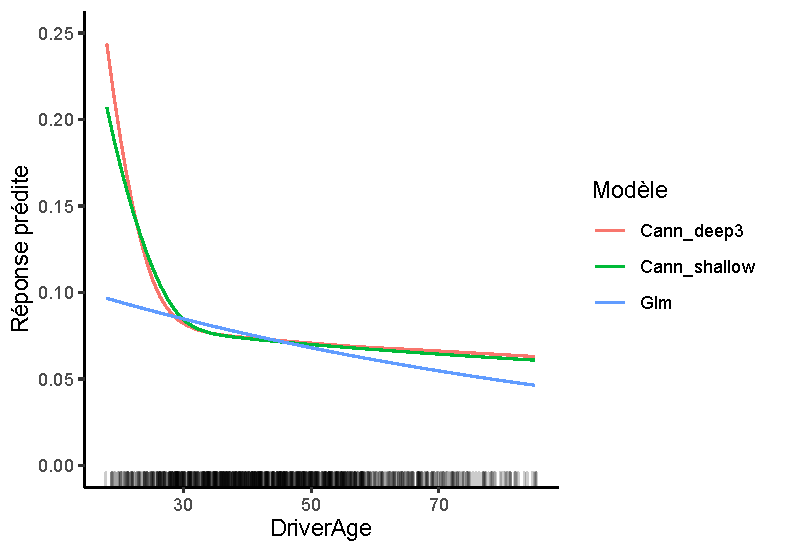
\includegraphics[scale=0.9]{Graphiques/pdp3modDriverAge}
\end{figure}




La \autoref{fig:pdp3CarAge} montre bien une différence entre les deux réseaux. Comme on le constatait à la \autoref{fig:ExpoTotFreqMoyCarAge}, le modèle CannDeep3 fait ressortir une augmentation de la fréquence prédite pour les véhicules âgés de 5 à 10 ans. Les deux autres modèles ne captent pas cet effet.


\begin{figure}
\centering
\caption{\label{fig:pdp3CarAge} Dépendance partielle pour la variable CarAge pour les trois modèles sélectionnés }
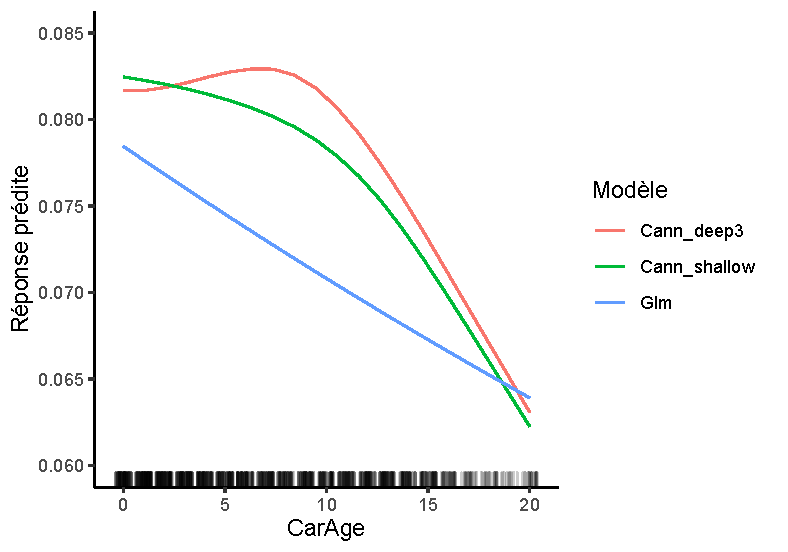
\includegraphics[scale=0.9]{Graphiques/pdpMod3CarAge}
\end{figure}

\begin{figure}
\caption{\label{fig:ice3Car} ICE pour la variable CarAge pour les trois modèles sélectionnés}
\centering
\begin{minipage}{0.45\linewidth}
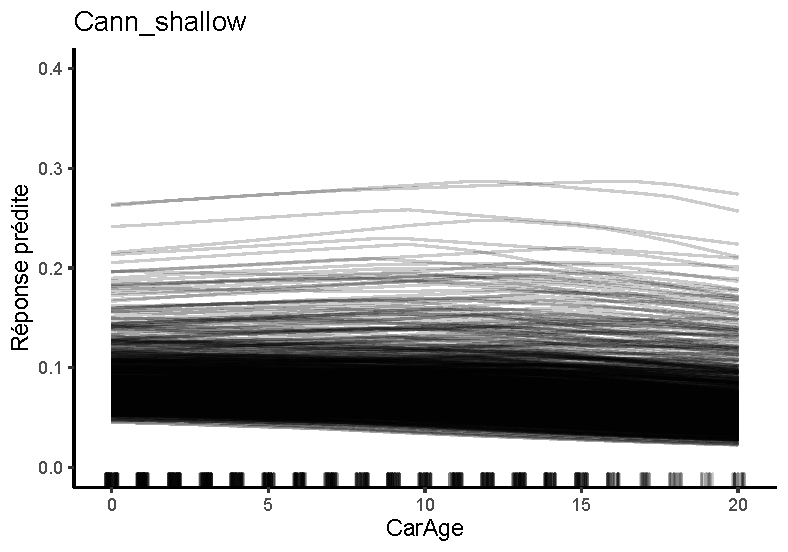
\includegraphics[scale=0.6]{Graphiques/iceCarShallow}
\end{minipage}
\hfill
\begin{minipage}{0.45\linewidth}
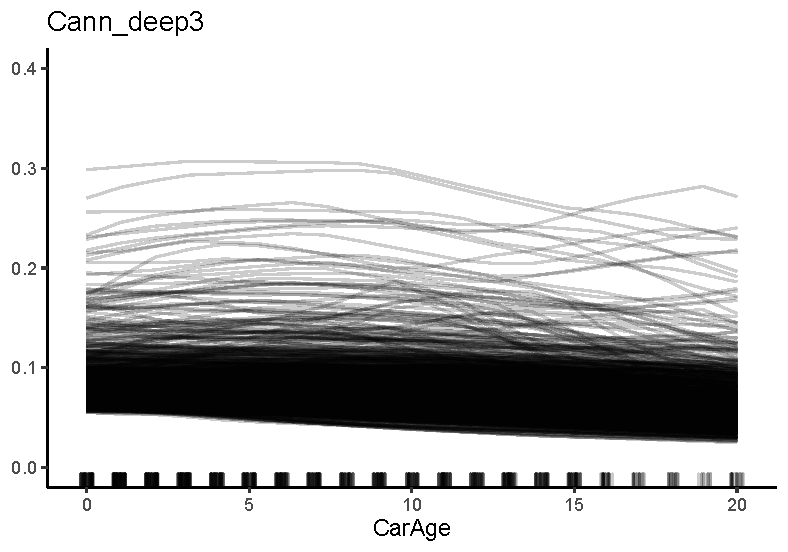
\includegraphics[scale=0.6]{Graphiques/iceCarCann}
\end{minipage}
\hfill
\begin{minipage}{0.45\linewidth}
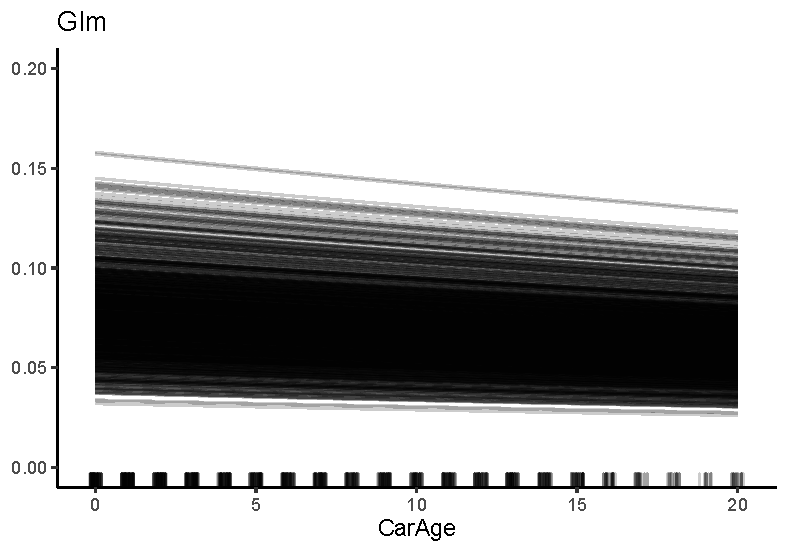
\includegraphics[scale=0.6]{Graphiques/iceCarGlm}
\end{minipage}
\end{figure}



L'effet de la variable \verb=Density= est plus difficile à distinguer. On voit clairement que la densité de la population fait augmenter le risque de réclammation pour ce portefeuille dans les trois modèles. Il semble avoir une légère différence pour le modèle CannDeep3 dans les extrémités de la courbe. Elle a une forme en « S », tandis que les deux autres courbes ne sont que convexes.

\begin{figure}
\centering
\caption{\label{fig:pdp3Density} Dépendance partielle pour la variable Density pour les trois modèles sélectionnés sur l'échelle logarithmique }
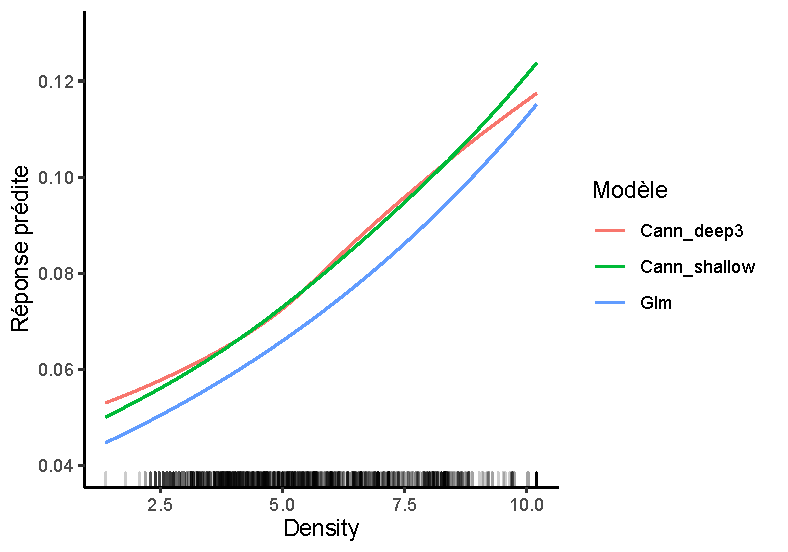
\includegraphics[scale=0.9]{Graphiques/pdp3ModDensity}
\end{figure}


La \autoref{fig:ice3Density} montre que le modèle CannDeep3 semble capter une interaction puisqu'on observe deux types de courbes. Le modèle prédit une légère augmentation pour une $log(Density)$ de 5 à 10 pour la plupart des assurés. Il y a cependant une certaine quantité d'assurés dont la prévision augmente rapidement pour des valeurs de 0 à 5 pour ensuite se stabiliser.

\begin{figure}
\caption{\label{fig:ice3Density} ICE pour la variable Density pour les trois modèles sélectionnés}
\centering
\begin{minipage}{0.45\linewidth}
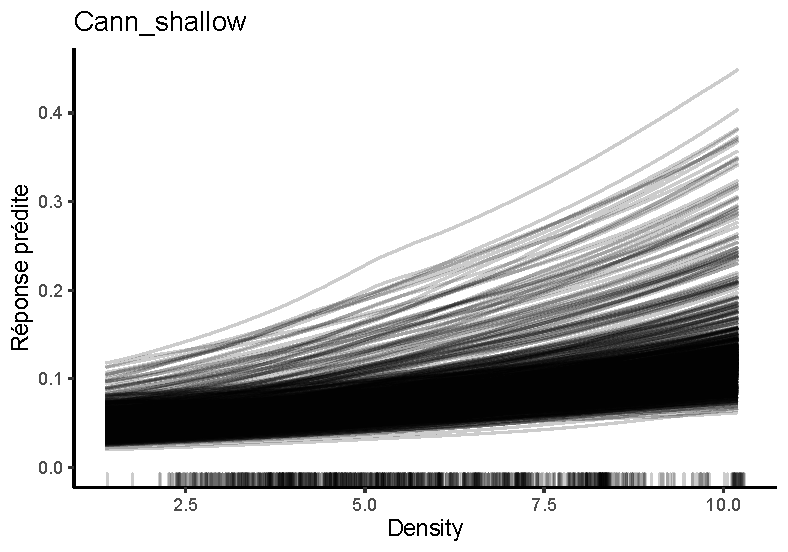
\includegraphics[scale=0.6]{Graphiques/iceDensityShallow}
\end{minipage}
\hfill
\begin{minipage}{0.45\linewidth}
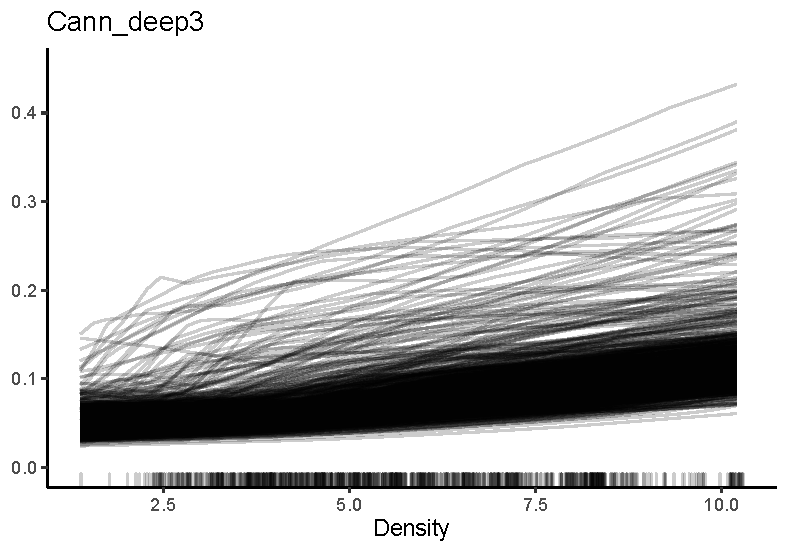
\includegraphics[scale=0.6]{Graphiques/iceDensityCann}
\end{minipage}
\hfill
\begin{minipage}{0.45\linewidth}
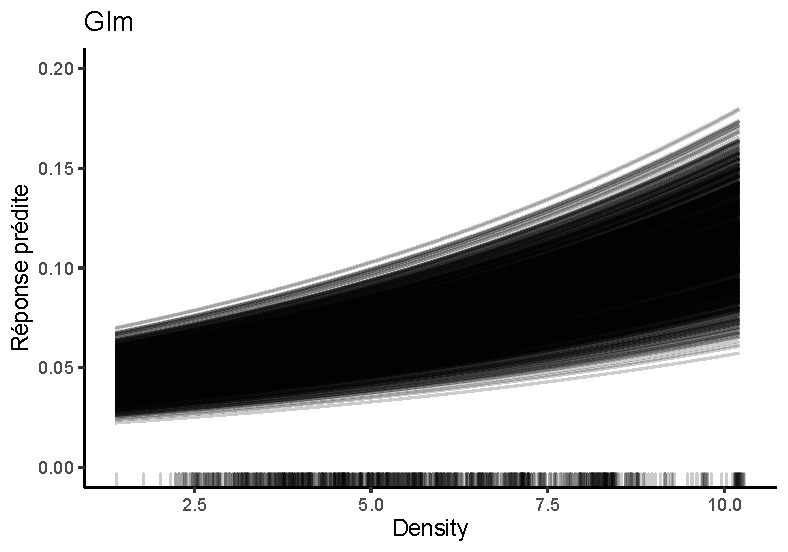
\includegraphics[scale=0.6]{Graphiques/iceDensityGlm}
\end{minipage}
\end{figure}


On observe à la \autoref{fig:interCann} que l'interaction de la variable \verb=Gas= avec les autres variables est la plus importante pour le modèle CannDeep3. Pour le modèle CannShallow, il s'agit de la variabe \verb=DriverAge=, \autoref{fig:interShallow}. On note plusieurs différences entre les deux modèles. Premièrement, le modèle CannDeep3 semble détecter plus d'interaction. Il y a cinq variables sur sept qui ont une statistique H supérieure à 0.2, tandis que le second réseau n'en compte que trois. Une autre différence notable est l'importance accordée aux interactions avec la variable \verb=DriverAge=. Le réseau profond la classe en cinquième position et le réseau à une couche la classe en première position. 


\begin{figure}
\centering
\caption{\label{fig:interCann} Interactions entre les variables explicatives pour le modèle CannDeep3 calculées à partir de la statistique H}
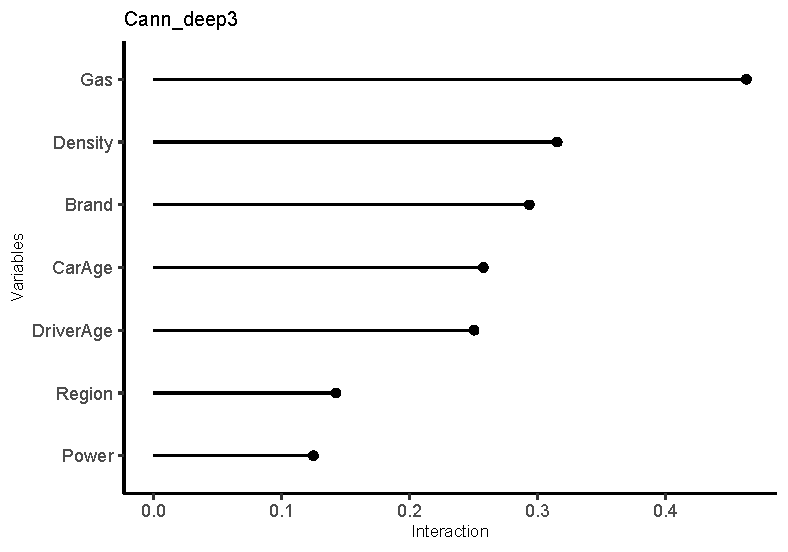
\includegraphics[scale=0.9]{Graphiques/interCann}
\end{figure}


\begin{figure}
\centering
\caption{\label{fig:interShallow} Interaction entre les variables explicatives pour le modèle CannShallow }
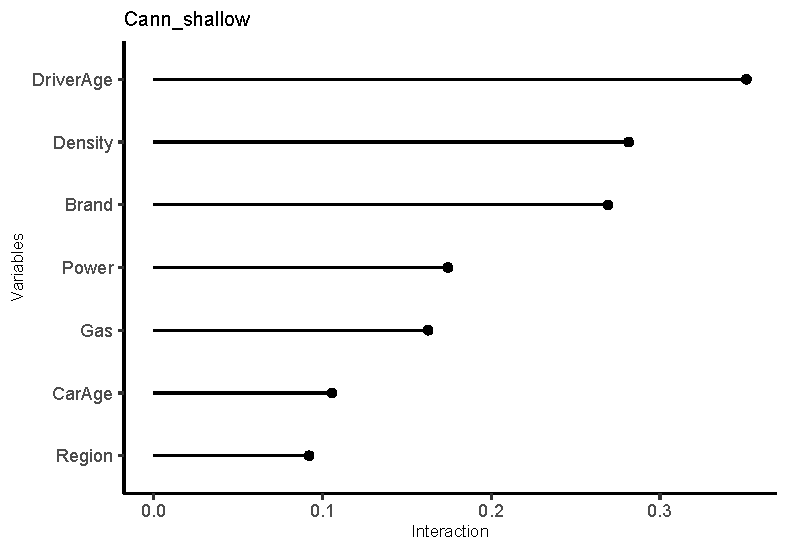
\includegraphics[scale=0.9]{Graphiques/interShallow}
\end{figure}

Les interactions avec la variable \verb=Gas= sont semblables pour les deux modèles. On note une seule différence notable pour l'interaction entre \verb=Density= et \verb=Gas=, où on obtient une statistique H à 0.2 pour le modèle CannDeep3 et 0.15 pour CannShallow.

\begin{figure}
\caption{\label{fig:inter3Gas} Interaction entre la variable Gas et les autres variables explicatives pour les modèles CannDeep3 et CannShallow}
\centering
\begin{minipage}{0.45\linewidth}
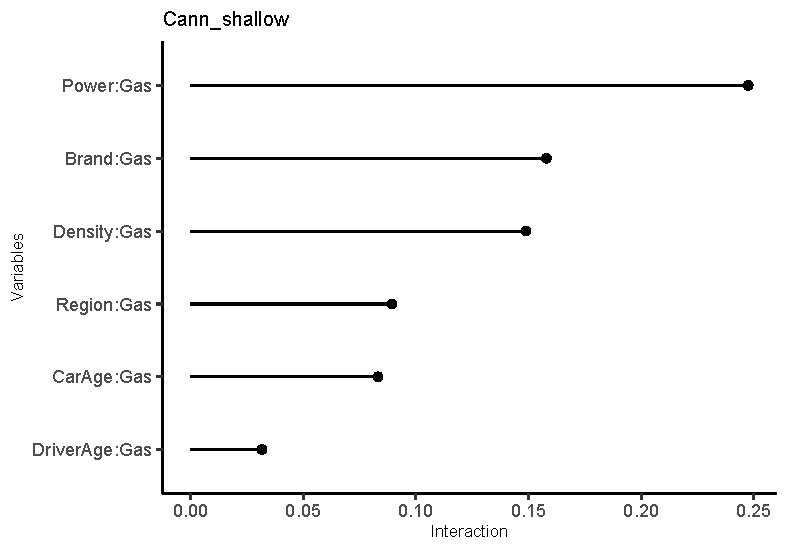
\includegraphics[scale=0.6]{Graphiques/interGasShallow}
\end{minipage}
\hfill
\begin{minipage}{0.45\linewidth}
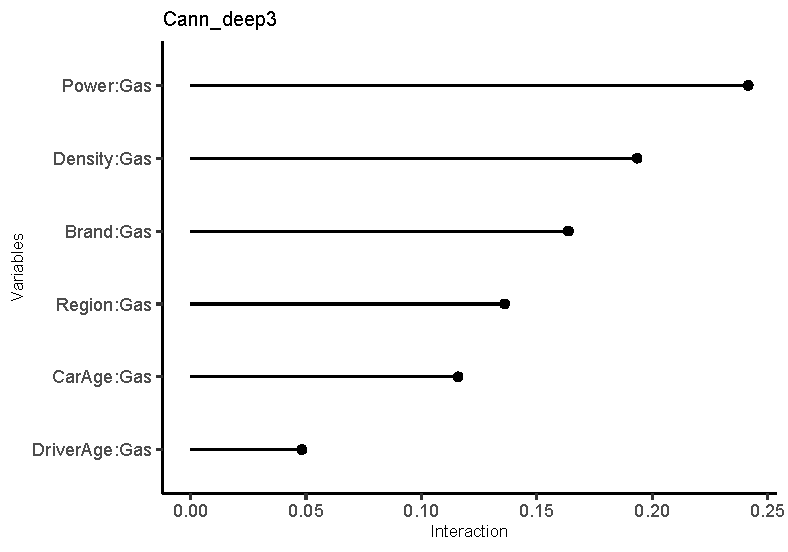
\includegraphics[scale=0.6]{Graphiques/interGasCann}
\end{minipage}
\end{figure}


On saisit mieux à l'aide de la \autoref{fig:inter3CarBrand} la raison possible de l'augmentation de la fréquence prédite des véhicules âgés de 5 à 10 ans par le modèle CannDeep3. On voit qu'il y a une interaction avec les véhicules japonnais. La courbe de cette marque de véhicule est clairement différente. Les autres marques ont toutes une diminution de la fréquence entre les âges mentionnés. Le réseau à une couche ne capte aucunement cet interaction. 

\begin{figure}
\caption{\label{fig:inter3CarBrand} Dépendance partielle entre les variables CarAge et Brand pour les trois modèles}
\centering
\begin{minipage}{0.45\linewidth}
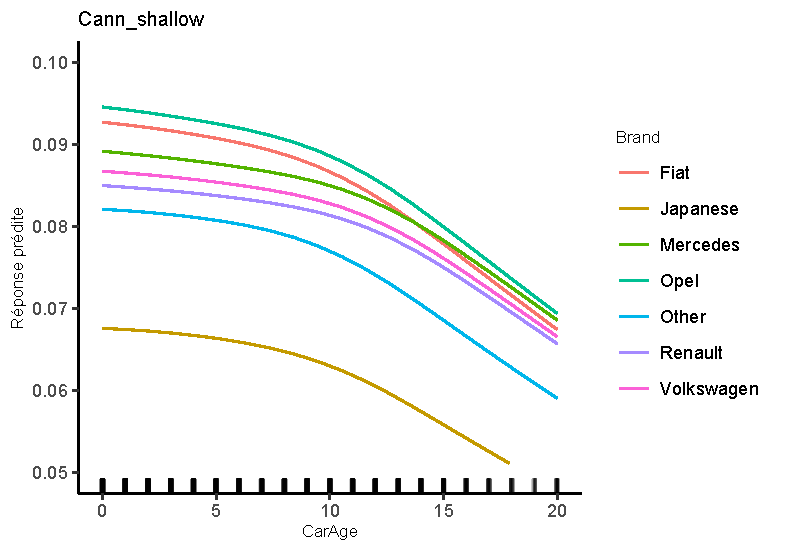
\includegraphics[scale=0.6]{Graphiques/interBrandCarShallow}
\end{minipage}
\hfill
\begin{minipage}{0.45\linewidth}
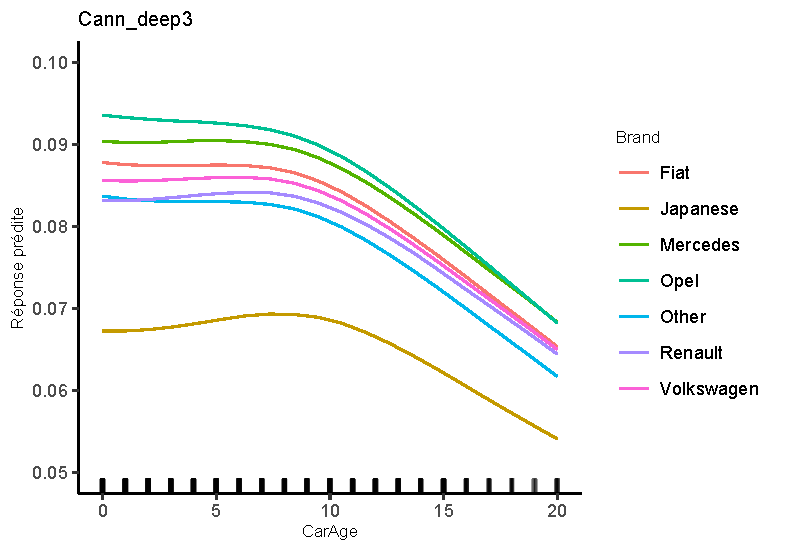
\includegraphics[scale=0.6]{Graphiques/interCarBrandCann}
\end{minipage}
\hfill
\begin{minipage}{0.45\linewidth}
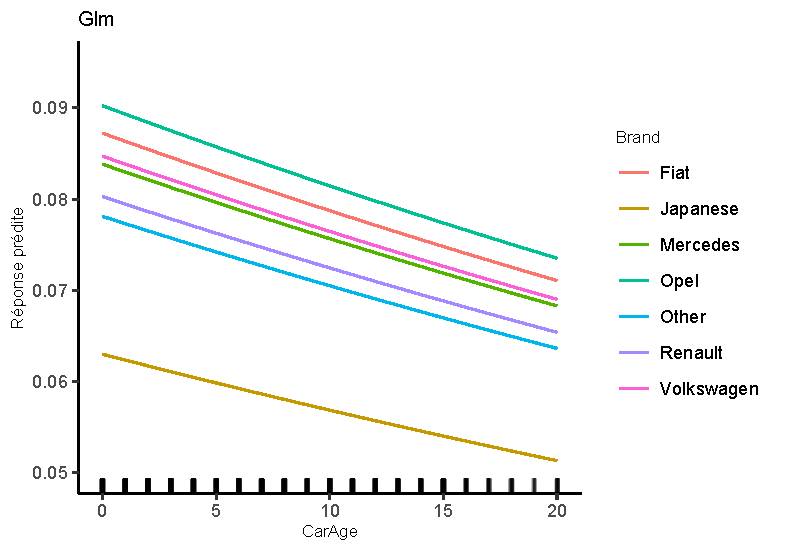
\includegraphics[scale=0.6]{Graphiques/interBrandCarGlm}
\end{minipage}
\end{figure}

On regarde maintenant les interactions avec \verb=DriverAge=. La \autoref{fig:inter3Driver} montre pour les deux modèles que les interactions avec \verb=Brand= et \verb=Density= sont les plus significatives. On illustre le PDP bivarié de \verb=DriverAge= et \verb=Density= à la \autoref{fig:inter3DriveDensity}. On y voit une différence pour les plus jeunes âges. Le modèles CannDeep3 prédit des fréquences élevées pour de jeunes conducteurs (environ moins de 25 ans) en combinaison avec une $log(Density)$ de 2.5 et plus. Le modèle CannShallow prédit des fréquences élevées pour de jeunes conducteurs, aussi, mais seulement pour une $log(Density)$ plus grande que 7.5 environ.

\begin{figure}
\caption{\label{fig:inter3Driver} Interaction entre la variable DriverAge et les autres variables explicatives pour les trois modèles}
\centering
\begin{minipage}{0.45\linewidth}
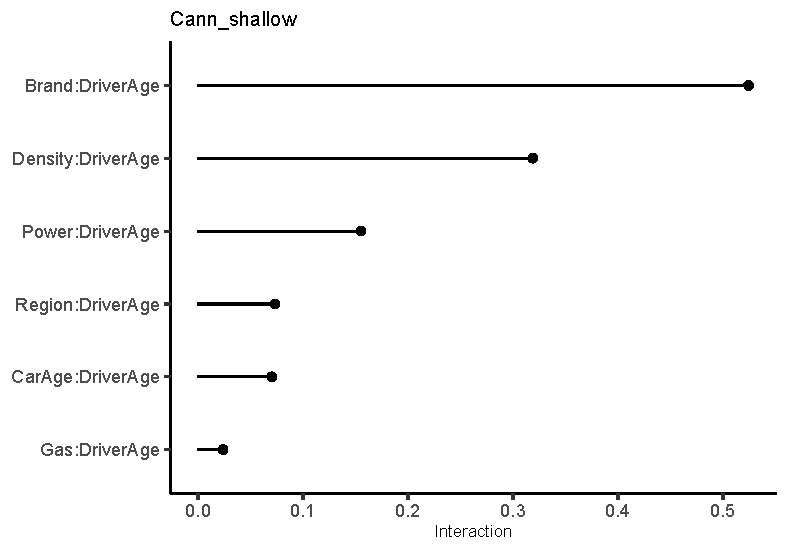
\includegraphics[scale=0.6]{Graphiques/interDriverAgeShallow}
\end{minipage}
\hfill
\begin{minipage}{0.45\linewidth}
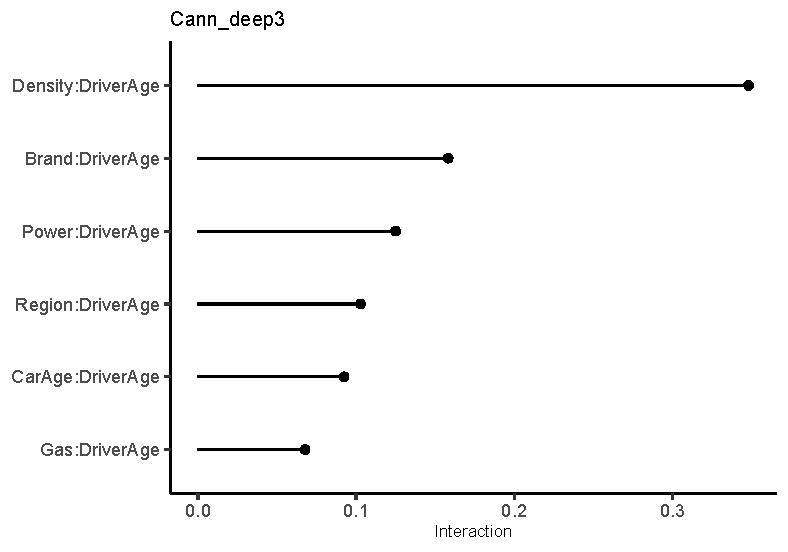
\includegraphics[scale=0.6]{Graphiques/interDriverAgeCann}
\end{minipage}
\end{figure}

\begin{figure}
\caption{\label{fig:inter3DriveDensity} Dépendance partielle entre les variables DriverAge et Density pour les trois modèles}
\centering
\begin{minipage}{0.45\linewidth}
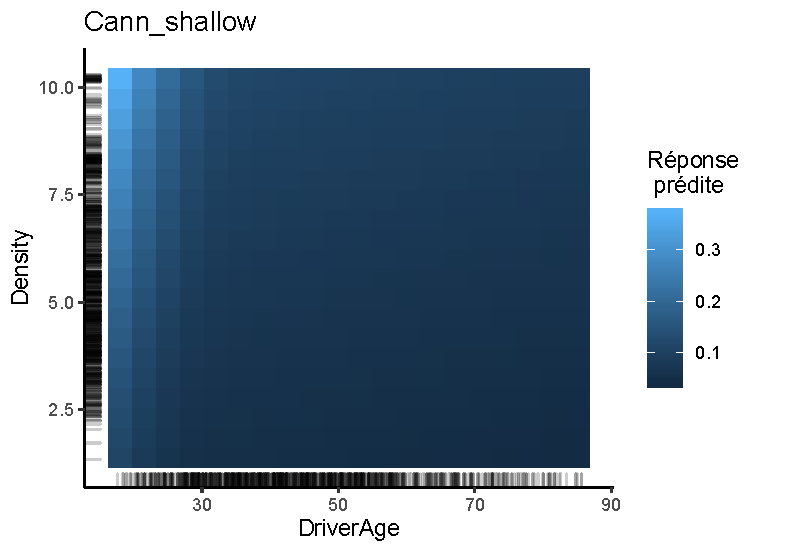
\includegraphics[scale=0.6]{Graphiques/interDriverDensityShallow}
\end{minipage}
\hfill
\begin{minipage}{0.45\linewidth}
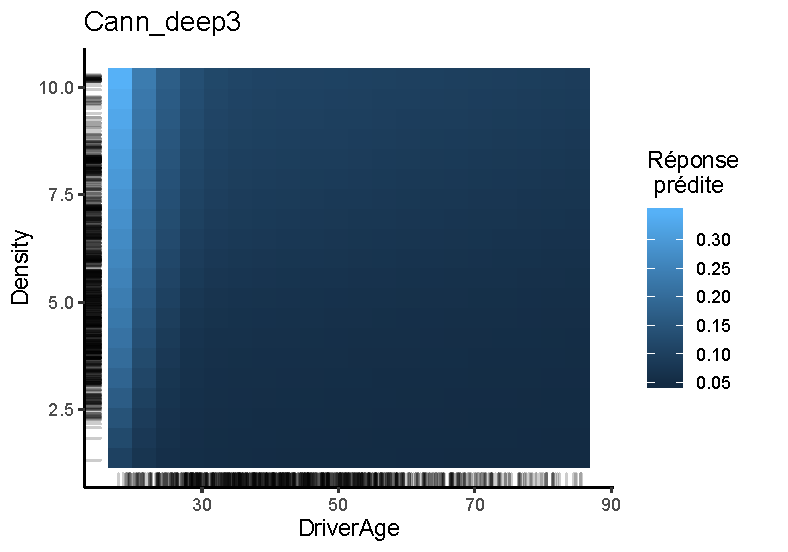
\includegraphics[scale=0.6]{Graphiques/interDriveDensityCann}
\end{minipage}
\hfill
\begin{minipage}{0.45\linewidth}
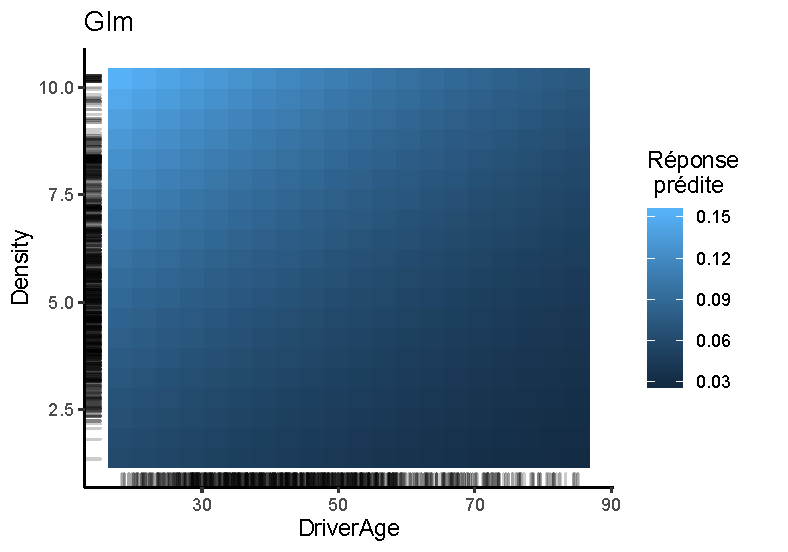
\includegraphics[scale=0.6]{Graphiques/interDriverDensityGlm}
\end{minipage}
\end{figure}